\subsection{Kn U claw}
La familia consiste en un grafo Kn y un grafo claw o estrella formado por un nodo y m nodos adyacentes, 
unidos de forma disjunta, que es luego complementado.
\begin{figure}[H]
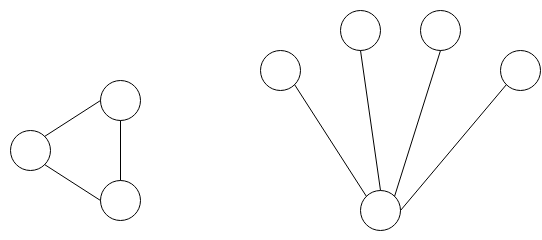
\includegraphics[width=80mm]{K3UC4.png}
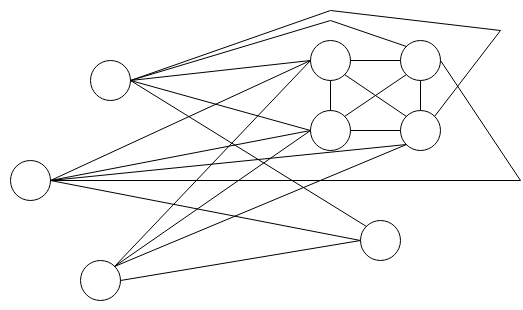
\includegraphics[width=80mm]{K3UC4Complemento.png}
\caption{La figura de la izquierda corresponde a K3 U claw 4, la figura derecha K3 U claw 4 complemento}
\label{overflow}
\end{figure}